\begin{exercice*}[Longueurs proportionnelles]
    Pour chaque figure : 
    \begin{itemize}
        \item Nommer les triangles dont les longueurs
        
        proportionnelles.
        \item Écrire les proportions égales
    \end{itemize}

    \emoji{light-bulb} Les droites en pointillés rouges sont paralléles.

    % \begin{multicols}2
        \begin{enumerate}
            \item \phantom{rrr}
            
            \begin{tikzpicture}[scale = 0.7]
                % \draw[help lines, color=black!30, dashed] (0,0) grid (10,7);        
                \coordinate[label=above:$A$] (A) at (1,6);
                \coordinate[label=above:$T$] (T) at (3.26,2.24);
                \coordinate[label=below:$S$] (S) at (4,1);
                \coordinate[label=above:$C$] (C) at (7.01,4.5);
                \coordinate[label=above:$R$] (R) at (9,4);
                \draw (A)--(S)--(R)--(A);
                \draw (T)--(C);                                
                \tkzDrawLine[dashed, color=red, ultra thick](T,C);
                \tkzDrawLine[dashed, color=red, ultra thick](S,R);
            \end{tikzpicture}
            \columnbreak

            \item \phantom{rrr}
                        
            \begin{tikzpicture}[scale = 0.7]
                % \draw[help lines, color=black!30, dashed] (0,0) grid (10,7);        
                \coordinate[label=above left:$R$] (R) at (5,6);
                \coordinate[label=above left:$T$] (T) at (3.01,1.5);
                \coordinate[label=above:$S$] (S) at (5,2);
                \coordinate[label=above:$U$] (U) at (1,5);
                \coordinate[label=right:$V$] (V) at (3.67,3);
                \tkzDrawLine(U,S);
                \tkzDrawLine(T,R);
                \tkzDrawLine(U,R);
                \tkzDrawLine(T,S);
                \tkzDrawLine[dashed, color=red, thick](U,R);
                \tkzDrawLine[dashed, color=red, thick](T,S);
            \end{tikzpicture}
        \end{enumerate}
    % \end{multicols}    
\end{exercice*}
\begin{corrige}
    %\setcounter{partie}{0} % Pour s'assurer que le compteur de \partie est à zéro dans les corrigés
    \phantom{rrr}    
    \begin{multicols}2
        \begin{enumerate}
            \item \phantom{rrr}
            
            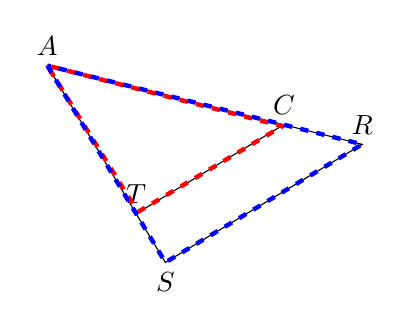
\begin{tikzpicture}[scale = 0.5]
                % \draw[help lines, color=black!30, dashed] (0,0) grid (10,7);        
                \coordinate[label=above:$A$] (A) at (1,6);
                \coordinate (A1) at (1,6);
                \coordinate[label=above:$T$] (T) at (3.26,2.24);
                \coordinate (T1) at (3.3,2.28);
                \coordinate[label=below:$S$] (S) at (4,1);
                \coordinate[label=above:$C$] (C) at (7.01,4.5);
                \coordinate (C1) at (6.97,4.46);
                \coordinate[label=above:$R$] (R) at (9,4);
                \draw (A)--(S)--(R)--(A);
                \draw (T)--(C);                                
                \draw[dashed, color=red, ultra thick](T1)--(C1)--(A1)--(T1);
                \draw[dashed, color=blue, ultra thick](A)--(S)--(R)--(A);
            \end{tikzpicture}
            
            Dans cette configuration, les droites $(TC)$ et $(SR)$ sont parallèles et les droites $(TS)$ et $(RC)$
            sont sécantes en $A$ donc :            

            \begin{itemize}
                \item Les triangles $\textcolor{red}{ATC}$ et $\textcolor{blue}{ASR}$ ont leurs longueurs proportionnelles.
                
                \item $\dfrac{\textcolor{red}{AT}}{\textcolor{blue}{AS}}=\dfrac{\textcolor{red}{AC}}{\textcolor{blue}{AR}}=\dfrac{\textcolor{red}{TC}}{\textcolor{blue}{SR}}$.
            \end{itemize}               
            
            \item \phantom{rrr}
            
            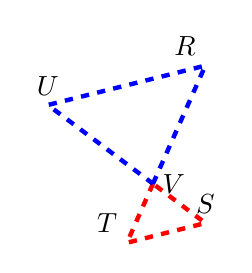
\begin{tikzpicture}[scale = 0.5]
                % \draw[help lines, color=black!30, dashed] (0,0) grid (10,7);        
                \coordinate[label=above left:$R$] (R) at (5,6);
                \coordinate[label=above left:$T$] (T) at (3.01,1.5);
                \coordinate[label=above:$S$] (S) at (5,2);
                \coordinate[label=above:$U$] (U) at (1,5);
                \coordinate[label=right:$V$] (V) at (3.67,3);
                \tkzDrawLine(U,S);
                \tkzDrawLine(T,R);
                \tkzDrawLine(U,R);
                \tkzDrawLine(T,S);
                \draw[dashed, color=red, ultra thick](V)--(T)--(S)--(V);
                \draw[dashed, color=blue, ultra thick](V)--(R)--(U)--(V);
            \end{tikzpicture}

            Dans cette configuration, les droites $(UR)$ et $(TS)$ sont parallèles et les droites $(US)$ et $(RT)$
            sont sécantes en $V$ donc :            

            \begin{itemize}
                \item Les triangles $\textcolor{blue}{RUV}$ et $\textcolor{red}{VTS}$ ont leurs longueurs proportionnelles.
                
                \item $\dfrac{\textcolor{red}{TV}}{\textcolor{blue}{RV}}=\dfrac{\textcolor{red}{VS}}{\textcolor{blue}{VU}}=\dfrac{\textcolor{red}{ST}}{\textcolor{blue}{RU}}$.
            \end{itemize}  
        \end{enumerate}
    \end{multicols}
\end{corrige}

